% +++
% latex="texfot lualatex-dev"
% +++
\documentclass[aspectratio=149,9pt,fleqn]{beamer}
\usetheme[numbering=fraction,block=fill]{metropolis}
\usefonttheme{professionalfonts}

\usepackage{luatexja,luatexja-adjust}
\usepackage[no-math,match,deluxe]{luatexja-fontspec}

\hypersetup{unicode,colorlinks}
\hypersetup{linkcolor=blue,urlcolor=teal,citecolor=olive}
% \hypersetup{linkcolor=black,urlcolor=black,citecolor=black}

\usepackage{pxrubrica}
\usepackage{autobreak}
\usepackage{tikz,pgfplots,tcolorbox}
\usetikzlibrary{calc}
\pgfplotsset{compat=1.16}

\usepackage[version=4,arrows=pgf]{mhchem}
\mhchemoptions{textfontcommand=\sffamily,mathfontcommand=\mathsf}
\newcommand*\cec[1]{\cesplit{{\,\ }{\0}}{#1}}

\usepackage{tabularray}
\SetTblrDefault{rowsep=0pt}

\usepackage[loadonly,]{enumitem}
\newlist{desc}{description}{5}
\setlist[desc]{labelindent=2\zw,labelsep*=1\zw,labelwidth=4\zw}
\newlist{enu}{enumerate}{5}
\setlist[enu]{label*=\arabic*.}

\ltjsetparameter{jacharrange={-2,-3,-8}}
\usepackage[no-math,match,deluxe,fontspec]{luatexja-preset}

% \usepackage[osf]{newpxtext}\usepackage{classico}
\usepackage[nowidering]{yhmath}
\usepackage{newpxmath,amsmath,mathtools,amssymb,mleftright}
\usepackage[T1]{fontenc}
\usepackage[notrig,italicdiff]{physics}
\mleftright

\usepackage[cal=boondoxo,frak=pxtx,bb=ams]{mathalpha}
\DeclareMathAlphabet{\mathnormal}{T1}{pplx}{m}{it}
\DeclareMathAlphabet{\mathrm}{T1}{pplx}{m}{n}
\DeclareMathAlphabet{\mathit}{T1}{pplx}{m}{it}
\DeclareMathAlphabet{\mathtt}{T1}{lmtt}{m}{n}
\DeclareMathAlphabet{\mathsf}{T1}{kurier}{m}{n}
\DeclareMathAlphabet{\mathbsf}{T1}{kurier}{b}{n}
\DeclareMathAlphabet{\mathbold}{T1}{pplx}{b}{it}
\DeclareMathAlphabet{\mathbf}{T1}{pplx}{b}{n}
\DeclareSymbolFont{operators}{T1}{uop}{m}{n}

\DeclareSymbolFont{numbers}{T1}{pplx}{m}{n}
\DeclareMathSymbol{0}\mathalpha{numbers}{`0}
\DeclareMathSymbol{1}\mathalpha{numbers}{`1}
\DeclareMathSymbol{2}\mathalpha{numbers}{`2}
\DeclareMathSymbol{3}\mathalpha{numbers}{`3}
\DeclareMathSymbol{4}\mathalpha{numbers}{`4}
\DeclareMathSymbol{5}\mathalpha{numbers}{`5}
\DeclareMathSymbol{6}\mathalpha{numbers}{`6}
\DeclareMathSymbol{7}\mathalpha{numbers}{`7}
\DeclareMathSymbol{8}\mathalpha{numbers}{`8}
\DeclareMathSymbol{9}\mathalpha{numbers}{`9}

\DeclareFontFamily{U}{mathastro}{}
\DeclareFontShape{U}{mathastro}{m}{n}{<->mathastrotest10}{}
\DeclareSymbolFont{astro}{U}{mathastro}{m}{n}
\DeclareMathSymbol\Sun\mathord{astro}{'300}
\DeclareMathSymbol\Mercury\mathord{astro}{'301}
\DeclareMathSymbol\Venus\mathord{astro}{'302}
\DeclareMathSymbol\Earth\mathord{astro}{'303}
\DeclareMathSymbol\Mars\mathord{astro}{'304}
\DeclareMathSymbol\Jupiter\mathord{astro}{'305}
\DeclareMathSymbol\Saturn\mathord{astro}{'306}
\DeclareMathSymbol\Uranus\mathord{astro}{'307}
\DeclareMathSymbol\Neptune\mathord{astro}{'310}
\DeclareMathSymbol\Pluto\mathord{astro}{'311}
\DeclareMathSymbol\varEarth\mathord{astro}{'312}
\DeclareMathSymbol\Moon\mathord{astro}{'313}
\DeclareMathSymbol\leftmoon\mathord{astro}{'313}
\DeclareMathSymbol\rightmoon\mathord{astro}{'314}
\DeclareMathSymbol\fullmoon\mathord{astro}{'315}
\DeclareMathSymbol\newmoon\mathord{astro}{'316}
\DeclareMathSymbol\newmoon\mathord{astro}{'316}

\setmainfont[
	Ligatures=TeX,
	Scale=0.98,
	BoldFont=FOT-RodinNTLGPro-B,
	ItalicFont=FOT-RodinNTLGPro-B,
]{Palatino}
\setsansfont[
	Ligatures=TeX,
	Scale=0.98,
	BoldFont=FOT-RodinNTLGPro-B,
	BoldItalicFont=FOT-RodinNTLGPro-B,
	%ItalicFont=FOT-RodinNTLGPro-B,
]{Palatino}
\setmainjfont[
	Ligatures=TeX,
	JFM=jlreq,
	BoldFont=FOT-RodinNTLGPro-B,
	ItalicFont=FOT-RodinNTLGPro-B,
]{FOT-ModeMinBLargePro-M}
\setsansjfont[
	Ligatures=TeX,
	JFM=jlreq,
	BoldFont=FOT-RodinNTLGPro-B,
	ItalicFont=FOT-RodinNTLGPro-B,
]{FOT-ModeMinBLargePro-M}
\setmonofont[
	Ligatures=TeXReset,
]{HackGen}
\setmonojfont[
	Ligatures=TeXReset,
]{HackGen}

\allowdisplaybreaks[4]
\ltjenableadjust[lineend=extended,priority=true,profile=true,linestep=false]

%%%%%%%%%%%%自作マクロ
\newcommand{\hmvec}{\mathbold}
\newcommand{\hmeqdef}{\stackrel{\mathrm{def}}{=}}
\newcommand{\hmeqq}{\stackrel{\mathrm{?}}{=}}
\newcommand{\centeralign}[1]{\rule{0pt}{0pt}\hfill#1\hfill\rule{0pt}{0pt}}
\NewDocumentCommand\hmu{s m}{\IfBooleanF{#1}{\,}\ifmmode\mathrm{#2}\else\(\mathrm{#2}\)\fi}
\newcommand{\hmemph}[1]{\textbf{#1}}
\newcommand{\hme}[1]{\times10^{#1}}
\newcommand{\hmfnc}[1]{\(\mathrm{#1}\)}
\newcommand{\hmfconv}{F_\mathrm{conv}}
\NewDocumentCommand\etal{s}{\textit{et al.}\IfBooleanF{#1}{\ }}

\institute{北海道大学大学院理学院 地球流体力学研究室 M2}
\author{人見祥磨}
\title{地球型惑星の射出限界の考察に向けて}
\subtitle{Ishiwatari \etal (2002) のレビュー}

\begin{document}

\maketitle

\begin{frame}
	\frametitle{背景}
	\begin{columns}[T,onlytextwidth]
		\begin{column}{.6\textwidth}
			\begin{itemize}
				\item 系外惑星に生命が存在するためには、惑星表面に液体の水があることが
					重要だと考えられる (Kopparapu \etal 2013)
				\item 惑星表面に液体の水が存在しうる領域は、ハビタブルゾーン (HZ)と呼ばれる
				\item 惑星表面に液体の水が存在する条件の一つは、惑星の表面温度が水の
					融点から沸点の間にあることである
				\item HZ の内側の、比較的高温な領域で起こる現象を考察する
			\end{itemize}
		\end{column}
		\begin{column}{.35\textwidth}
			\centering
			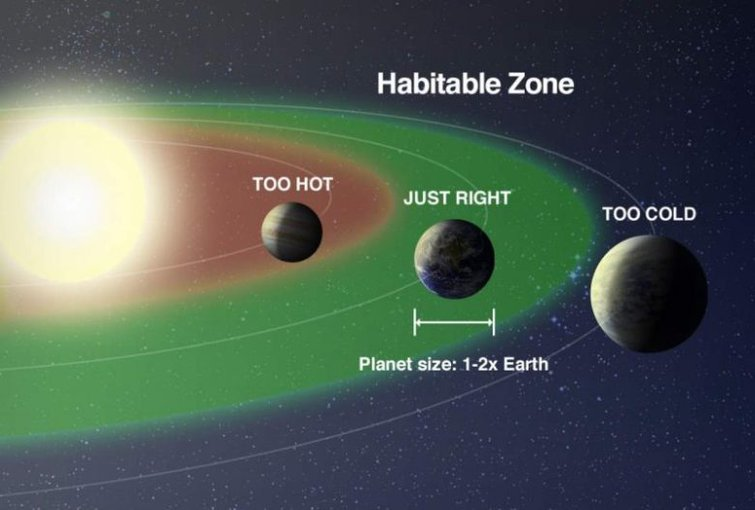
\includegraphics[width=\textwidth]{hz.jpg}\\
			\scriptsize HZ の概要図。Image credit: NASA
		\end{column}
	\end{columns}
\end{frame}

\begin{frame}
	\frametitle{暴走温室状態}
	\begin{itemize}
		\item HZ の内側境界を決定する重要な事象として、暴走温室状態が議論されている
	\end{itemize}
	\begin{columns}[T,onlytextwidth]
		\begin{column}{.65\textwidth}
			\begin{itemize}
				\item 様々なモデルで暴走温室状態の研究が進められていた
					\begin{itemize}
						\item 温度が上昇すると水蒸気量が増え、
							温室効果をもつ水蒸気が増大することでさらに地表面温度が上昇する、
							正のフィードバックによる温度が上昇し続け、海洋と大気が平衡に
							なれず、海洋が完全に蒸発する (Plass 1961 や Gold 1964)
						\item 灰色成層圏モデルを用い、惑星大気上端での外向き赤外放射
							(outgoing longwave radiation: OLR) には上限がある
							(Komabayashi, 1967, 1968; Ingersoll, 1969)
						\item 精密な放射過程・熱力学過程をもち、対流圏まで考慮したモデル
							でも放射上限があらわれる(Kasting 1988; Abe and Matsui 1988)
					\end{itemize}
				\item 暴走温室状態や射出限界について、Nakajima \etal (1992) が整理を行った
			\end{itemize}
		\end{column}
		\begin{column}{.3\textwidth}
			\centering\small
			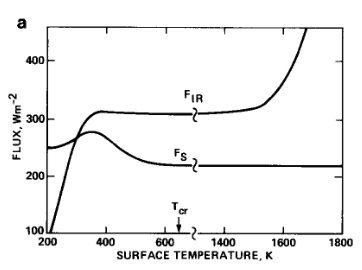
\includegraphics[width=.95\textwidth]{kasting7a.png}\\
			Kasting (1988) Fig.\ 7a\\
			精密モデルでの OLR (\(F_{\mathrm{IR}}\)) と\\
			地表面温度の関係
		\end{column}
	\end{columns}
\end{frame}

\begin{frame}
	\frametitle{Nakajima \etal (1992) のレビュー}
	\begin{itemize}
		\item Nakajima \etal (1992) は 1 次元放射対流平衡モデルを用いて
			OLR に 2 種類の上限があると示した
			\begin{itemize}
				\item 大気に水蒸気が極端に
					少ないときにあらわれる Komabayashi--Ingersoll Limit
				\item 対流圏の構造によって与えられる放射上限
					(Kastingや Abe and Matsui の上限に対応)
				\item このふたつの上限は異なる原因によるとわかった
			\end{itemize}
	\end{itemize}
	\begin{columns}[c]
		\begin{column}{.55\textwidth}
			\centering\small
			\begin{tblr}{rl}
				\hline
				&Nakajima \etal (1992) モデル設定\\
				\hline
				成層圏&放射平衡\\
				対流圏界面&飽和水蒸気\\
				対流圏&飽和断熱減率\\
				放射過程&散乱なし、灰色\\
				成分&理想気体、2 成分(水蒸気・乾燥空気)\\
				臨界点&なし\\
				\hline
			\end{tblr}
		\end{column}
		\begin{column}{.4\textwidth}
			\centering\small
			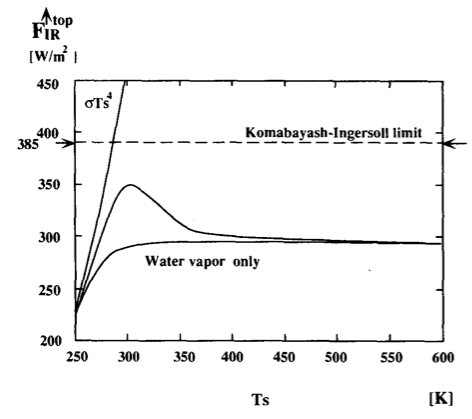
\includegraphics[width=\textwidth]{nf4.png}\\
			Nakajima \etal (1992) Fig.\ 3\\
			地表面温度と OLR の関係
		\end{column}
	\end{columns}
\end{frame}

\begin{frame}
	\frametitle{Ishiwatari \etal (2002) の目的}
	\begin{itemize}
		\item Nakajima \etal (1992) の枠組みを踏まえ 3 次元で行うことが目的
			\begin{itemize}
				\item 入射するエネルギーフラックス (surface shortwave radiation: SSR) の
					緯度分布も考慮した
				\item 3 次元で運動も取り入れた計算をした
				\item 時間発展計算を行う
					\begin{itemize}
						\item 平衡解が安定か検討できる
						\item 平衡解が存在しない場合の振る舞いを検討できる
					\end{itemize}
			\end{itemize}
	\end{itemize}
\end{frame}

\begin{frame}
	\frametitle{モデル設定}
	\begin{columns}[T,onlytextwidth]
		\begin{column}{.5\textwidth}
			\begin{itemize}
				\item 基本の設定は Nakajima \etal (1992) と同一
					\begin{itemize}
						\item 大気は凝結性成分(水蒸気)と非凝結性成分(乾燥空気)からなる
						\item 両成分とも分子量が同じであるとする
						\item 水蒸気のみが長波放射を吸収し、灰色であるとする
					\end{itemize}
				\item 地表面で熱バランスが成り立ち、湿り度は 1 とする(すべて海で覆われている)
				\item 平分解能は三角形切断の T21 に対応した \(32\times64\)
			\end{itemize}
		\end{column}
		\begin{column}{.45\textwidth}
			\tiny\centering
			\begin{tblr}{rl}
				\hline
				&モデル設定\\
				\hline
				成層圏&放射平衡\\
				対流圏&飽和断熱減率\\
				放射過程&散乱なし、灰色\\
				成分&理想気体、水蒸気・乾燥空気\\
				臨界点&なし\\
				\hline
				\hline
				気体定数&\(R=8.314\hmu{J/kg/K}\)\\
				重力加速度&\(g=9.8\hmu{m/s^2}\)\\
				\hline
				非凝縮成分の分子量&\(m_n=18\hme{-3}\hmu{kg/mol}\)\\
				凝縮成分の分子量&\(m_v=18\hme{-3}\hmu{kg/mol}\)\\
				凝縮成分の定圧モル比熱&\(c_{pv}=3.5R\)\\
				非凝縮成分の定圧モル比熱&\(c_{pn}=3.5R\)\\
				凝縮成分の潜熱&\(L=2.4253\hme{6}\hmu{J/kg}\)\\
				飽和水蒸気曲線の定数&\(p^*_0=1.4\hme{11}\hmu{Pa}\)\\
				地表面での非凝縮成分の量&\(p_{n0}=10^5\hmu{Pa}\)\\
				凝縮成分の吸収係数&\(\kappa_v=0.01\hmu{m^2/kg}\)\\
				非凝縮成分の吸収係数&\(\kappa_n=0\hmu{m^2/kg}\)\\
				\hline
				地表面の比熱&\(0\)\\
				地表面のアルベド&\(0\)\\
				\hline
			\end{tblr}
		\end{column}
	\end{columns}
	\begin{columns}[T,onlytextwidth]
		\begin{column}{.5\textwidth}
			\begin{itemize}
				\item 太陽定数 \(S\) を変化させて実験を行った
					\begin{itemize}
						\item 実験した太陽定数は下表の 8 つ。実験名の S の後ろが太陽定数
						\item 実験 S1380 が現在の地球に相当
						\item 全球平均 SSR は \(S\) の \(1/4\)
					\end{itemize}
			\end{itemize}
		\end{column}
		\begin{column}{.45\textwidth}
			% \centering\small
			% 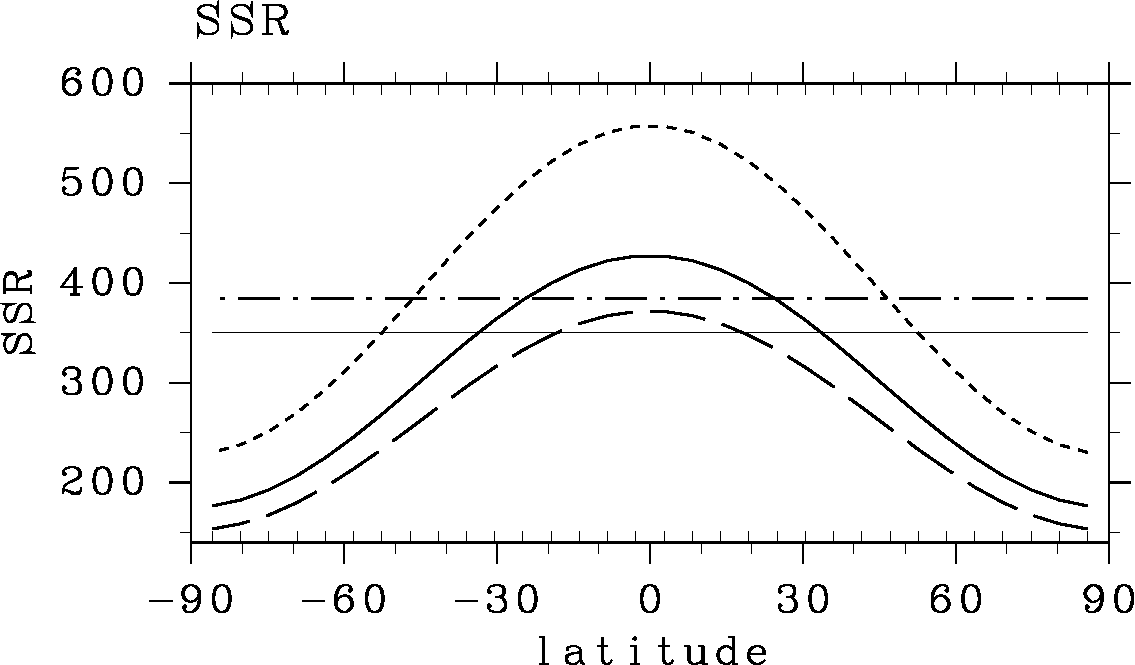
\includegraphics[width=.8\textwidth]{./fig/SSR.kps-crop.pdf}\\
			% Ishiwatari \etal (2002) Fig.~1\\
			% モデルに与える SSR の緯度分布と\\
			% Komabayashi--Ingersoll limit,\\
			% 及び Nakajima \etal (1992) で\\
			% 得られた放射上限 (\hmu*{W/m^2})
			\begin{table}
				\scriptsize
				実験を行った太陽定数
				\begin{tblr}{c|cccc}
					\hline
					実験名&S1200&S1380&S1500&S1550\\
					\hline
					SSR(\hmu*{W/m^2})&300.0&345.0&375.0&387.5\\
					\hline
					\hline
					実験名&S1570&S1600&S1700&S1800\\
					\hline
					SSR(\hmu*{W/m^2})&392.5&400.0&425.0&450.0\\
					\hline
				\end{tblr}
			\end{table}
		\end{column}
	\end{columns}
\end{frame}

\begin{frame}
	\frametitle{基礎方程式}
	\tiny
	\begin{gather*}
		\dv{\zeta}{t}=-\frac{1}{a\cos\varphi}\pdv{}{\lambda}
		\qty[-(\zeta+f)u-\dot\sigma\pdv{u}{\sigma}-\frac{RT'}{a\cos\varphi}\pdv{\pi}{\lambda}]
		-\frac{1}{a\cos\varphi}\pdv{}{\varphi}
		\qty[\qty((\zeta+f)v-\dot\sigma\pdv{u}{\sigma}-\frac{RT'}{a}\pdv{\pi}{\varphi})\cos\varphi]
		-F_\zeta^\mathit{diff},\tag{渦度}\\
		\dv{D}{t}=\frac{1}{a\cos\varphi}\pdv{}{\lambda}
		\qty[(\zeta+f)v-\dot\sigma\pdv{u}{\sigma}-x\frac{RT'}{a}\pdv{\pi}{\varphi}]
		+\frac{1}{a\cos\varphi}\pdv{}{\varphi}
		\qty[\qty((\zeta+f)v-\dot\sigma\pdv{u}{\sigma}-\frac{RT'}{a}\pdv{\pi}{\varphi})\cos\varphi]
		-\nabla^2(\Phi+R\bar T\pi+E)-F_D^\mathit{diff},\tag{発散}\\
		\dv{\pi}{t}=-\frac{1}{a\cos\varphi}\pdv{u}{\lambda}
		-\frac{1}{a\cos\varphi}\pdv{}{\varphi}[v\cos\varphi]-\pdv{\dot\sigma}{\sigma},\quad
		\pdv{\Phi}{\sigma}=-\frac{RT}{\sigma},\quad
		\dv{q}{t}=\frac{g}{p_s}\pdv{F_q^\mathit{vdf}}{\sigma}+F_q^\mathit{vdf}+S_q^\mathit{cond},
		\tag{連続の式, 静水圧, 比湿}\\
		\dv{T}{t}=\frac{RT}{c_p}\qty(\pdv{\pi}{t}+\frac{u}{a\cos\varphi}\pdv{\pi}{\lambda}+
		\frac{v}{a}\pdv{\pi}{\varphi}+\frac{\dot\sigma}{\sigma})
		+\frac{1}{c_p}\qty(\frac{g}{p_s}\pdv{F_T^\mathit{vdf}}{\sigma}+
		\frac{g}{p_s}\pdv{F_\mathrm{rad}^\mathit{vdf}}{\sigma})
		+F_T^\mathit{diff}+LS_q^\mathit{cond},\tag{熱力学}\\
		\dv{}{t}
		\equiv\pdv{}{t}+\frac{u}{a\cos\varphi}\pdv{}{\lambda}
		+\frac{u}{a}\pdv{}{\varphi}+\dot\sigma\pdv{}{\sigma},\quad
		\zeta\equiv\frac{1}{a\cos\varphi}\pdv{v}{\lambda}
		-\frac{1}{a\cos\varphi}\pdv{}{\varphi}[u\cos\varphi],\\
		D\equiv\frac{1}{a\cos\varphi}\pdv{u}{\lambda}
		+\frac{1}{a\cos\varphi}[v\cos\varphi],\quad
		\Phi\equiv gz,\quad\pi\equiv\ln p_s
	\end{gather*}
	\((\lambda,\varphi)\): 緯度経度; \(\sigma\): 高度(\(\sigma\) 座標); \(u, v\): 水平風;
	\(\dot\sigma\): \(\sigma\) 座標での鉛直風; \(T\): 温度; \(q\): 比湿;
	\(p_s\): 地表面気圧; \(f\): コリオリパラメータ; \(a\): 惑星半径; \(g\): 重力加速度;\\
	\(R\): 乾燥空気の気体定数; \(c_p\): 定圧比熱; \(L\): 水の潜熱;
	\(F_\bullet^\mathit{diff}\): 水平拡散項; \(F_\bullet^\mathit{vdf}\): 鉛直拡散項;
	\(S_q^\mathit{cond}\): 結露・凝結による比湿の変化;
\end{frame}

\begin{frame}
	\frametitle{Ishiwatari \etal (2002) の問題点}
	\begin{itemize}
		\item この計算に用いた GCM (AGCM) にはバグが含まれていた (Ishiwatari \etal (2021))
			\begin{itemize}
				\item 湿潤対流調節スキームが動作する条件が逆になっていた
				\item 鉛直成層が湿潤断熱減率よりも安定しているときに対流調節が働くようになっていた
			\end{itemize}
		\item 試計算を行ったところ、上層大気で内部重力波が増幅して、計算不安定が起きた
			\begin{itemize}
				\item 内部重力波に対して、強い人工的散逸を導入した
				\item ハドレー循環や傾圧不安定などの対流圏の大気循環の基本的な構造は表現
					されているので、大きな影響はないとした
			\end{itemize}
		\item 修士研究では、モデルのバグを修正した計算を行う予定
	\end{itemize}
\end{frame}

\begin{frame}
	\frametitle{熱的暴走状態の発生}
	\begin{figure}
		\scriptsize
		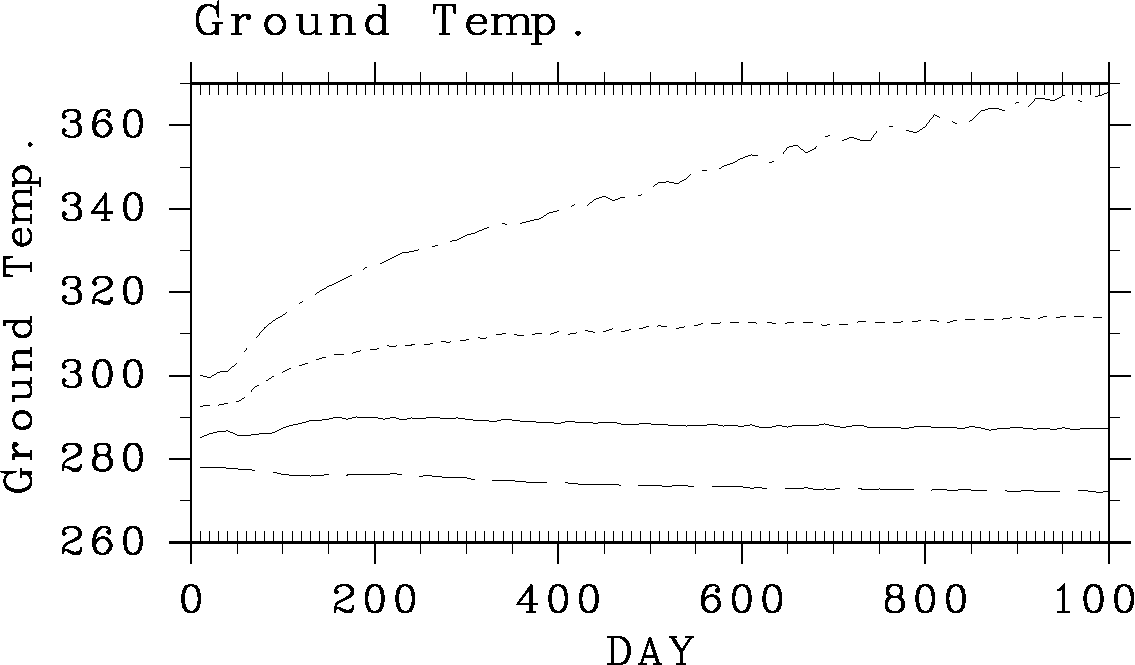
\includegraphics[width=.45\textwidth]{./fig/Tg-seqs.kps-crop.pdf}
		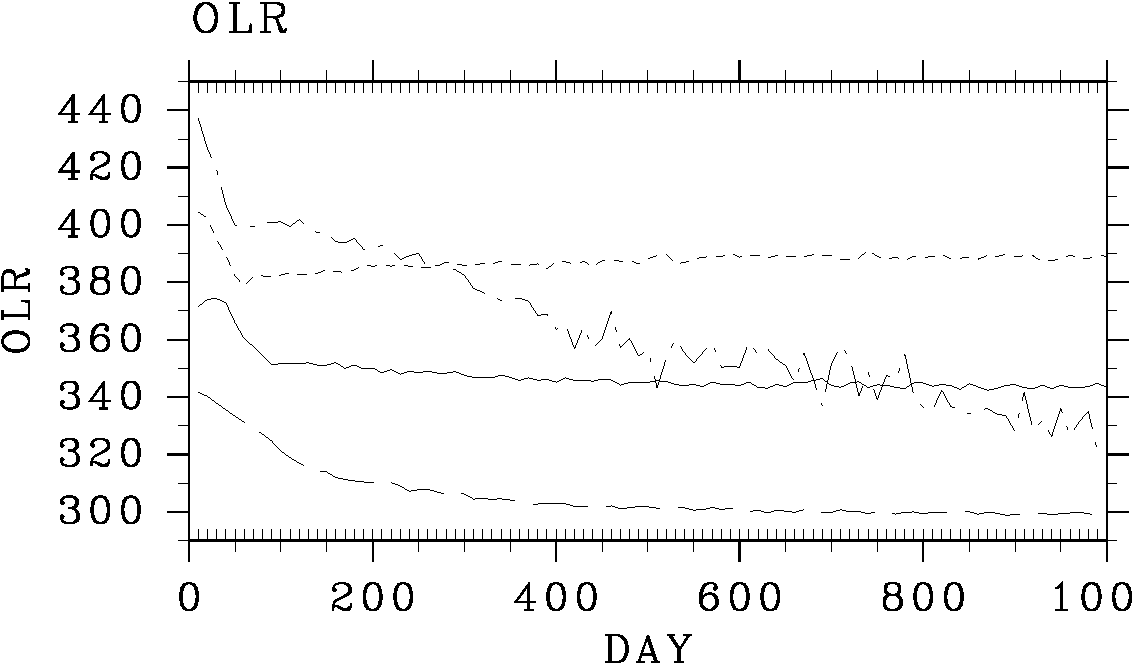
\includegraphics[width=.45\textwidth]{./fig/OLR-seqs.kps-crop.pdf}\\
		Ishiwatari \etal (2002) Fig.~2\\
		全球平均 OLR (\hmu*{W/m^2}) と全球平均表面温度 (\hmu*{K}) の時間変化\\
		S1200, S1380, S1570, S1800 の結果
	\end{figure}
	\begin{columns}[T,onlytextwidth]
		\begin{column}{.7\textwidth}
			\begin{itemize}
				\item \(S\leq1570\hmu{W/m^2}\) の場合、全球平均 OLR と全球平均 SSR が一致し、
					平衡状態になる
				\item \(S=1800\hmu{W/m^2}\) の場合、全球平均 SSR \(450\hmu{W/m^2}\) と全球平均
					OLR との差が広がり続け、平衡状態にならない
					\begin{itemize}
						\item OLR は減少し続け、表面温度は増加し続ける
					\end{itemize}
				\item \(S>1600\hmu{W/m^2}\) では平衡状態にならない
			\end{itemize}
		\end{column}
		\begin{column}{.3\textwidth}
			\centering\scriptsize
			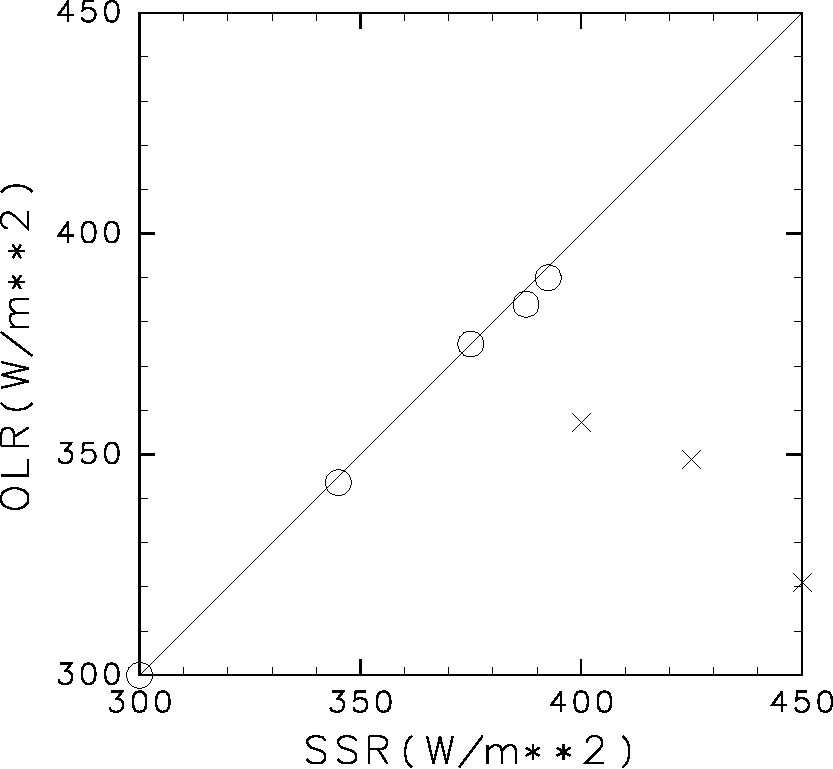
\includegraphics[width=.7\textwidth]{./fig/ISR-OLR.kps-crop.pdf}\\
			Ishiwatari \etal (2002) Fig.~3\\
			1000 日での SSR と OLR の関係\\
			(S1600 では 2000 日)\\
			◯では熱的平衡、×印では熱的暴走
		\end{column}
	\end{columns}
\end{frame}

\begin{frame}
	\frametitle{熱的暴走の発生}
	\begin{columns}[T,onlytextwidth]
		\begin{column}{.55\textwidth}
			\begin{itemize}
				\item 赤道付近の OLR は約 \(390\hmu{W/m^2}\) で頭打ち
				\item 中高緯度の OLR は太陽定数の増加に伴って \(400\hmu{W/m^2}\) に漸近
				\item 東西平均温度も OLR と同様に平坦化の傾向
				\item 以上から熱的平衡状態が得られる太陽定数の上限は概ね \(1600\hmu{W/m^2}\)
				\item これらが Nakajima \etal (1992) で指摘された放射上限に対応するものかを考察する
			\end{itemize}
		\end{column}
		\begin{column}{.4\textwidth}
			\centering
			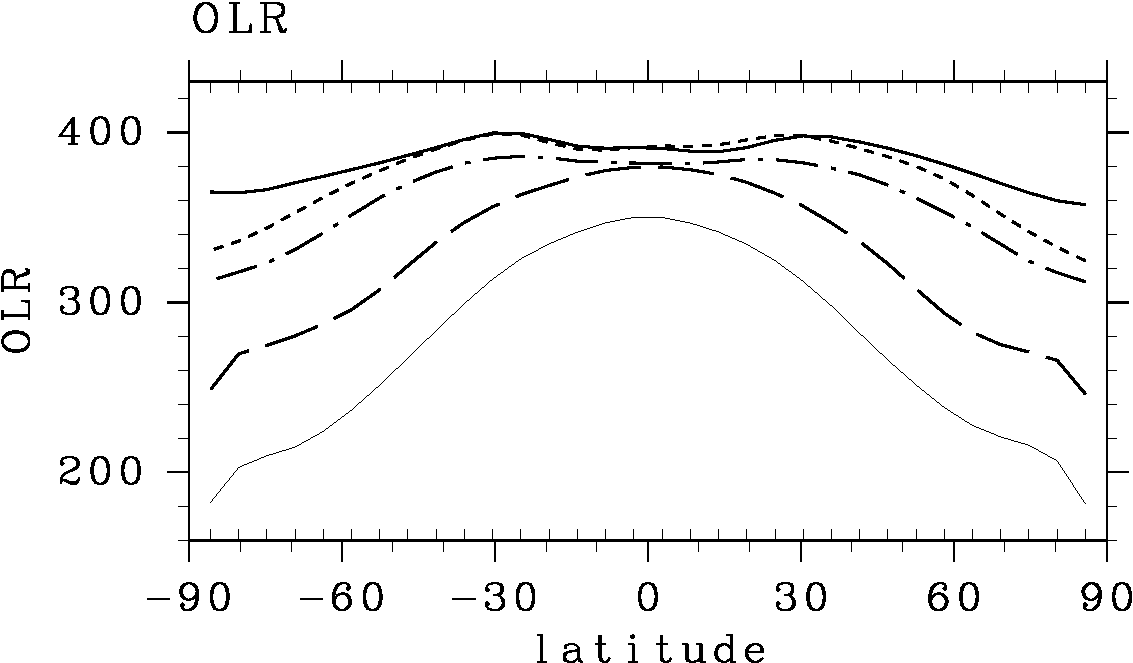
\includegraphics[width=\textwidth]{./fig/OLR-meris.kps-crop.pdf}\\
			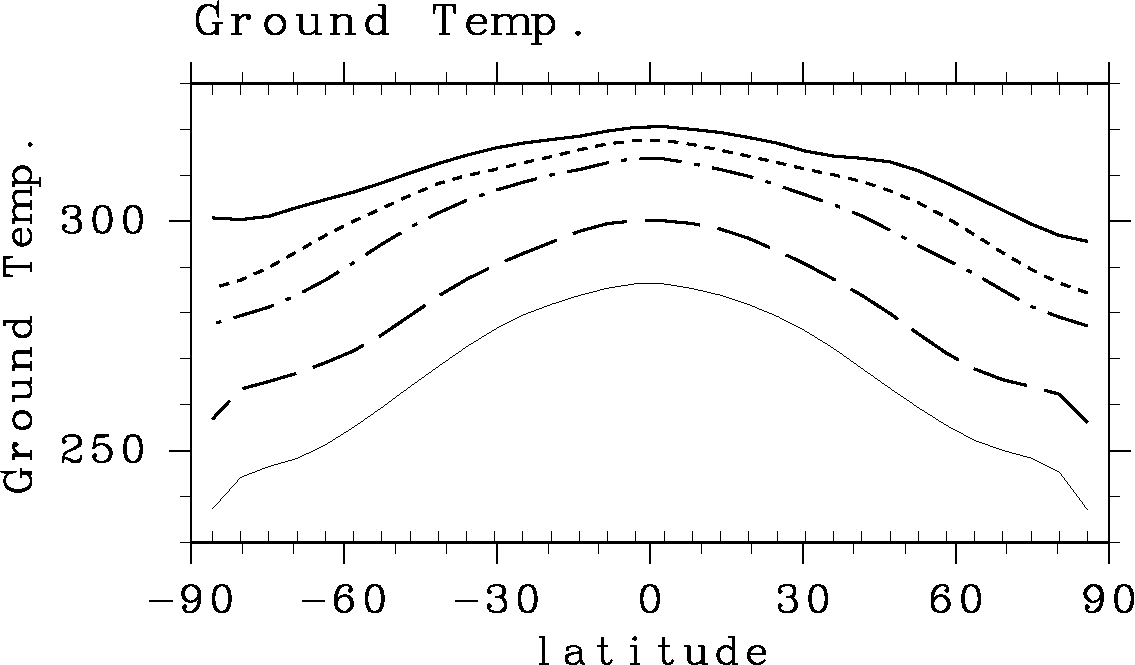
\includegraphics[width=\textwidth]{./fig/Tg-meris.kps-crop.pdf}\\
			\scriptsize Ishiwatari \etal (2002) Fig.\ 4\\
			平衡状態における OLR と東西平均値表面温度\\
			実験 S1570, S1550, S1500, S1380, S1200 の結果
		\end{column}
	\end{columns}
\end{frame}

\begin{frame}
	\frametitle{1 次元系との比較}
	\begin{columns}[T,onlytextwidth]
		\begin{column}{.45\textwidth}
			\begin{itemize}
				\item Komabayashi--Ingersoll limmit との対応
					\begin{itemize}
						\item 実験 S1570 では、圏界面の相対湿度は \(50\hmu{\%}\) 程度
						\item この場合の Komabayashi--Ingersoll limit を計算すると約 \(450\hmu{W/m^2}\) になる
						\item 得られた上限値より大きい
					\end{itemize}
				\item Nakajima \etal (1992) が得た放射上限との対応
					\begin{itemize}
						\item 実験 S1570 での赤道域対流圏相対湿度は \(60\hmu{\%}\) 程度
						\item 大気の相対湿度を \(60\hmu{\%}\) に固定して、1 次元放射対流平衡モデルで
							放射上限を計算すると、\(385\hmu{W/m^2}\)
						\item 得られた漸近値に近い
					\end{itemize}
			\end{itemize}
		\end{column}
		\begin{column}{.5\textwidth}
			\centering
			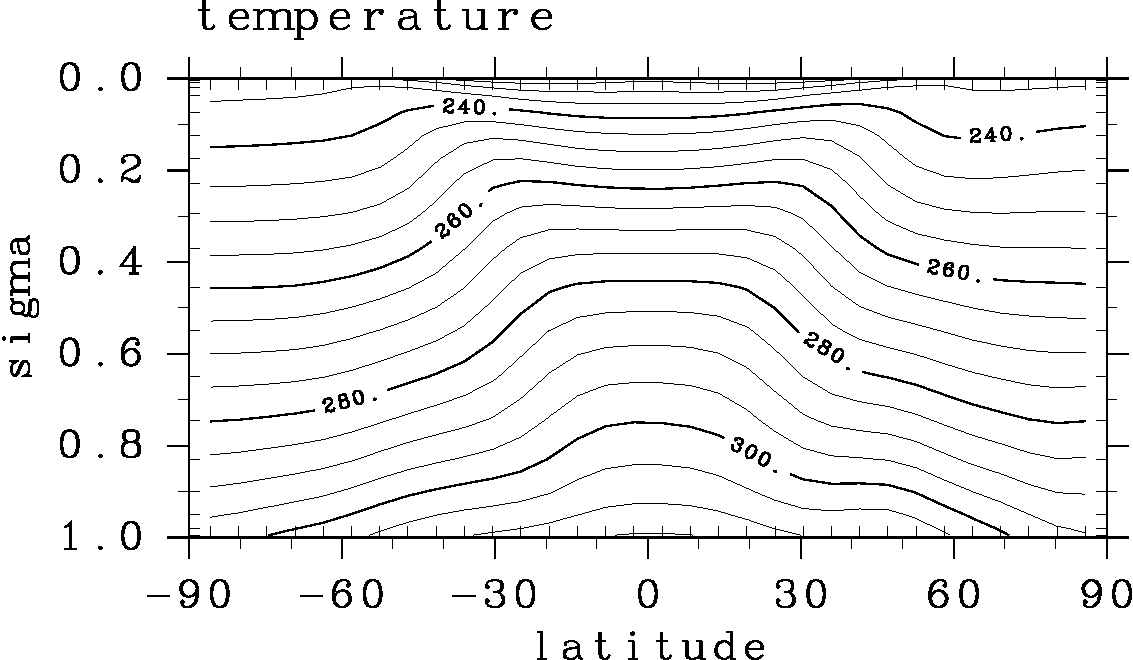
\includegraphics[width=.45\textwidth]{./fig/157-T-meri.kps-crop.pdf}
			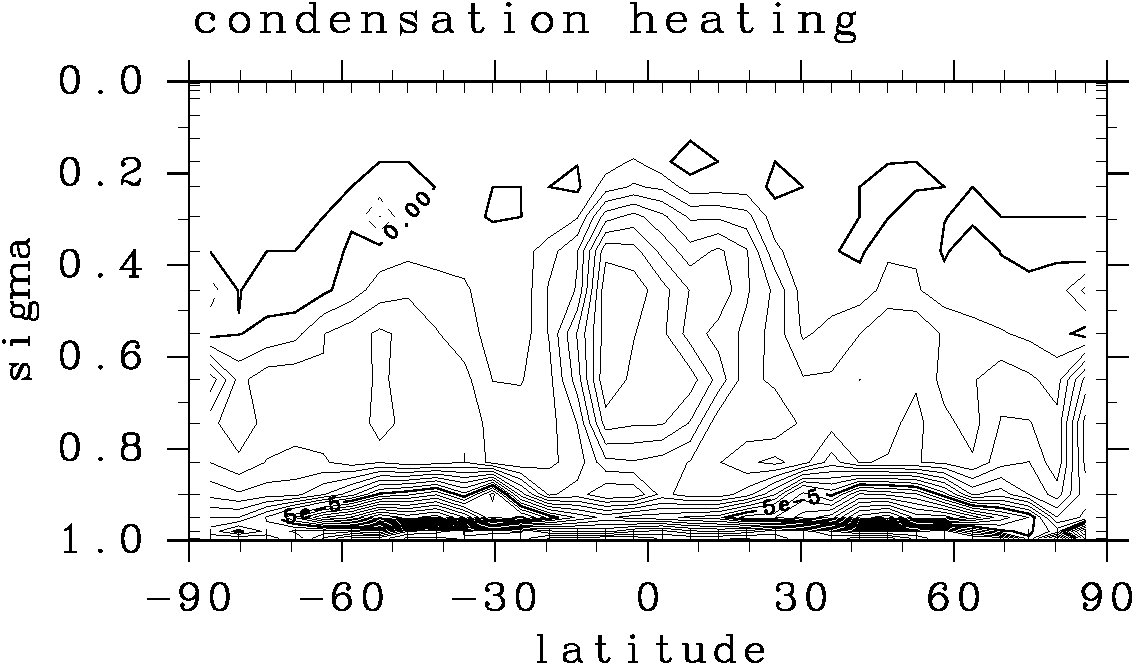
\includegraphics[width=.45\textwidth]{./fig/157-Qcnd-meri.kps-crop.pdf}
			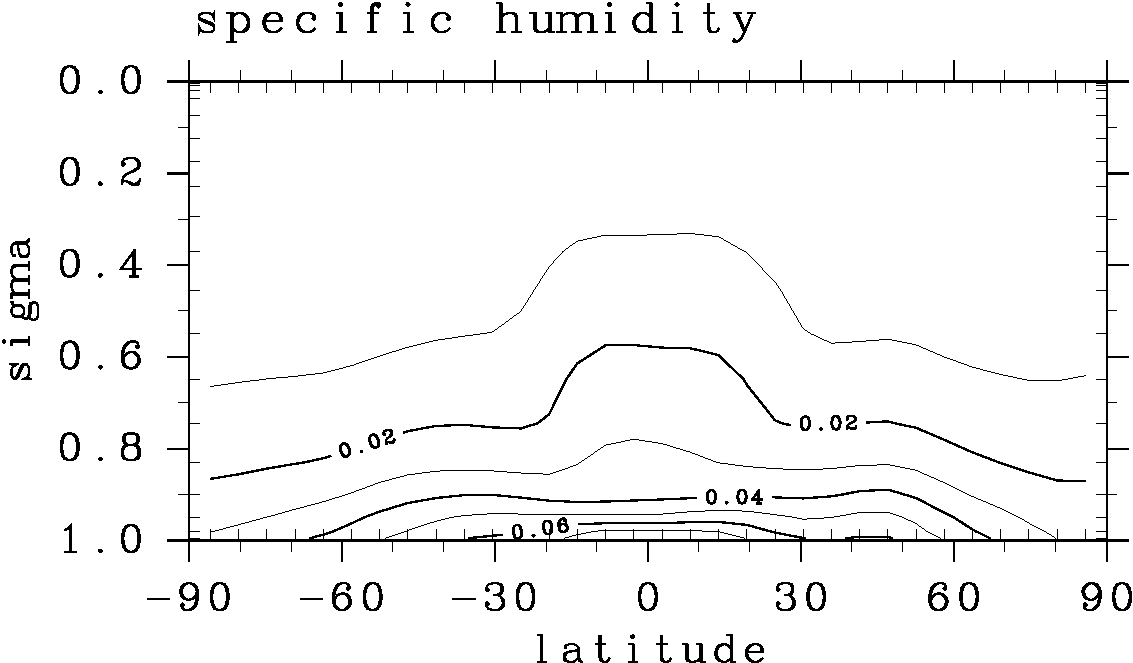
\includegraphics[width=.45\textwidth]{./fig/157-q-meri.kps-crop.pdf}
			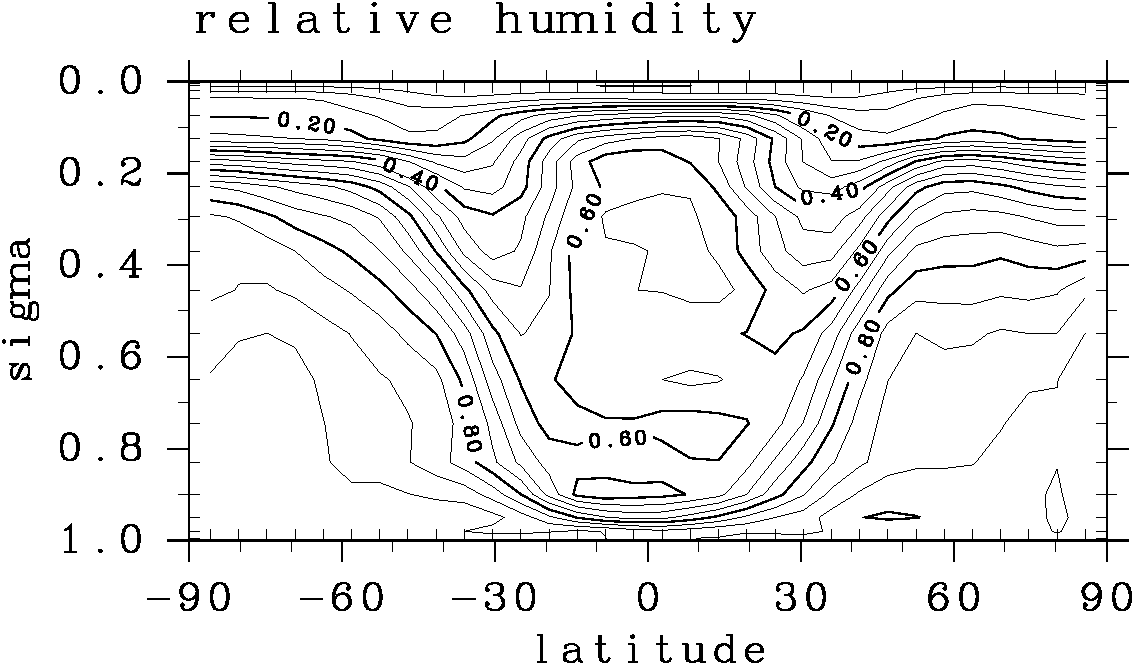
\includegraphics[width=.45\textwidth]{./fig/157-RH-meri.kps-crop.pdf}
			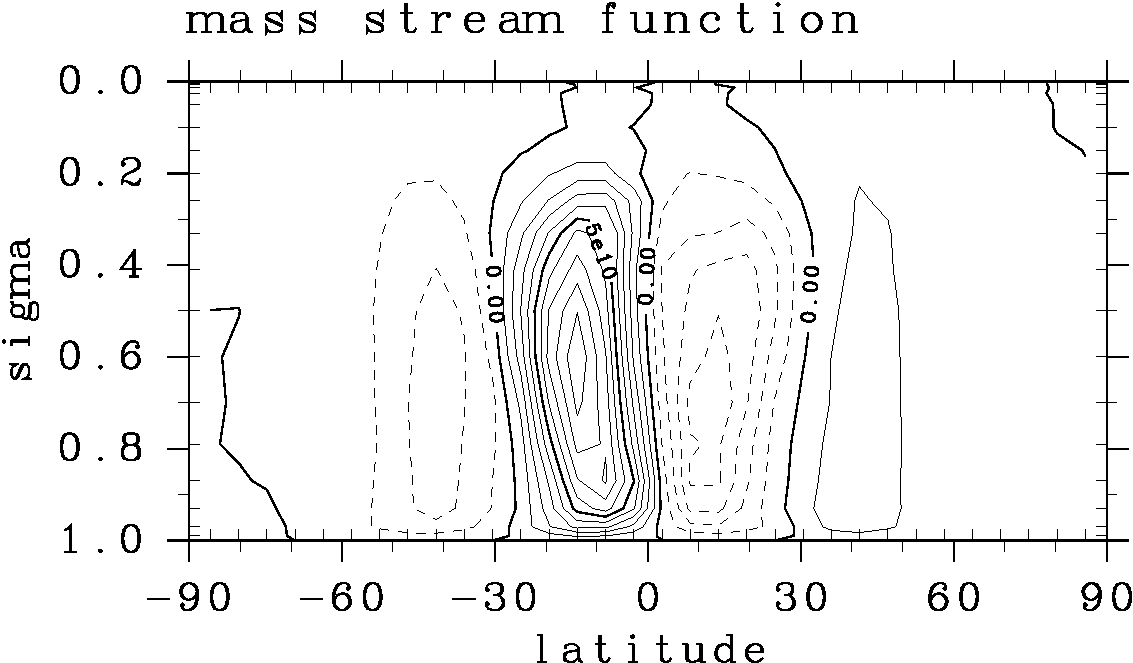
\includegraphics[width=.45\textwidth]{./fig/157-Strm-meri.kps-crop.pdf}
			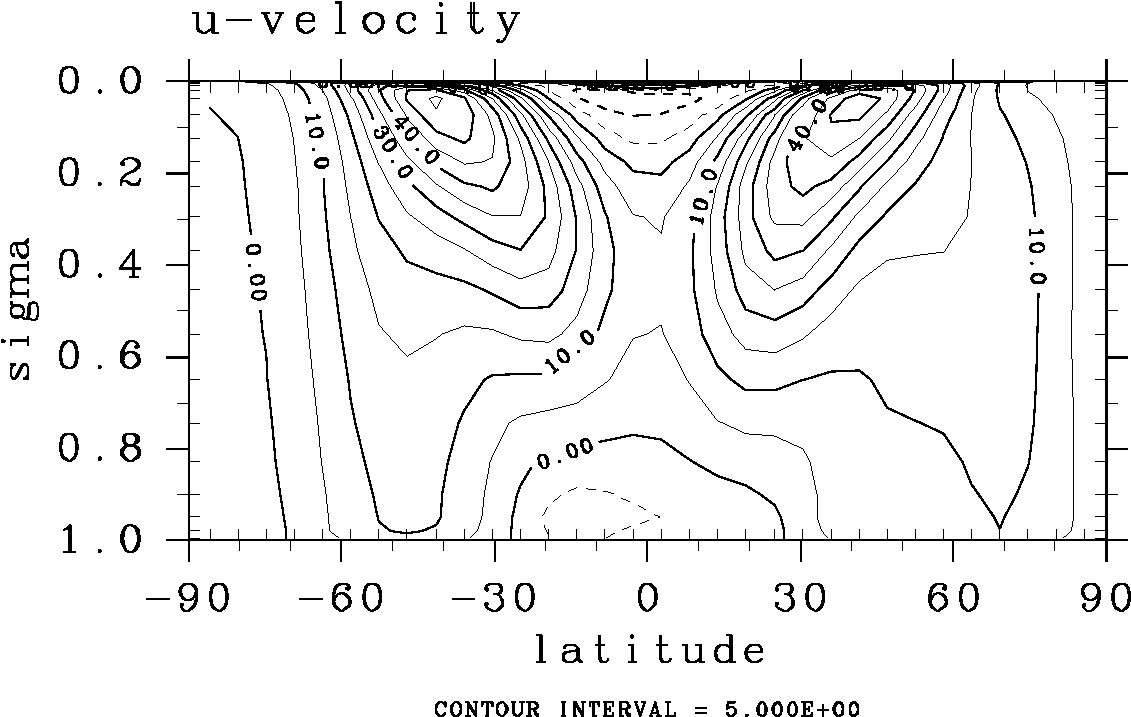
\includegraphics[width=.45\textwidth]{./fig/157-u-meri-crop.pdf}\\
			\scriptsize Ishiwatari \etal (2002) Fig.\ 9\\
			実験 S1570 の子午面構造\\
			温度・凝結加熱・比湿・相対湿度・質量流線関数・東西風
		\end{column}
	\end{columns}
\end{frame}

\begin{frame}
	\frametitle{1 次元系との比較}
	\begin{columns}[T,onlytextwidth]
		\begin{column}{.4\textwidth}
			\begin{itemize}
				\item 1 次元系で相対湿度を変化させて放射上限を求めてみる
				\item その結果は、3 次元計算と若干のずれはあるものの、対応を示しているように見える
				\item 前頁の結果からも、3 次元計算で得られた漸近値は、Nakajima \etal (1992)
					が得た放射上限に対応していると言える
			\end{itemize}
		\end{column}
		\begin{column}{.6\textwidth}
			\centering\scriptsize
			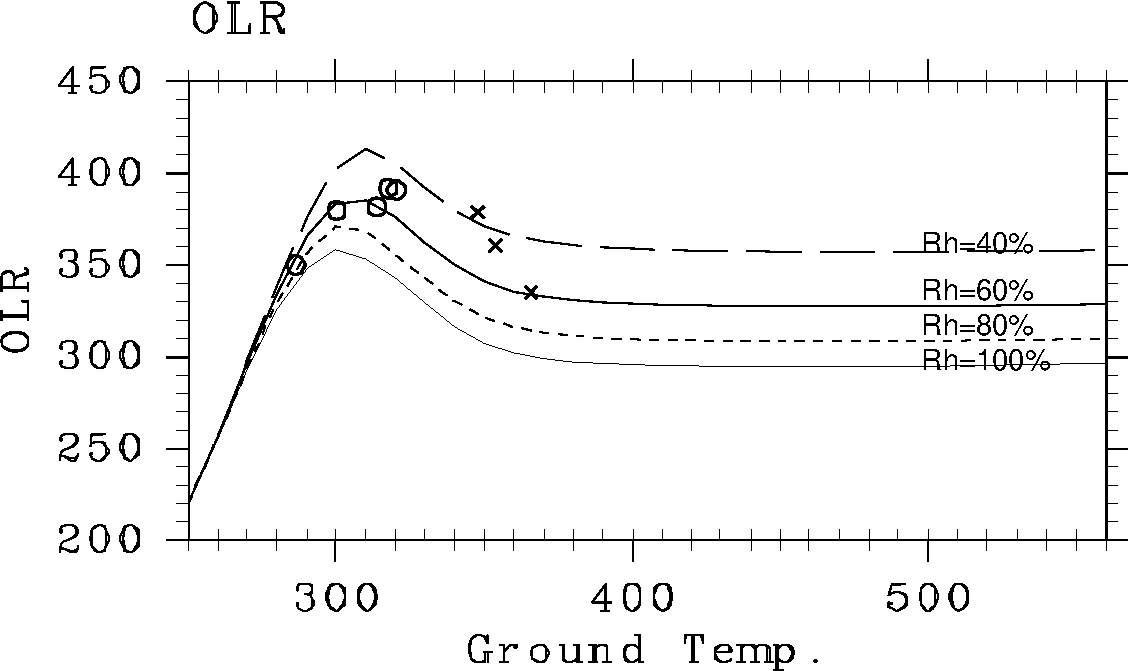
\includegraphics[width=.8\textwidth]{./fig/Tg-OLR-1dimL99-3dEq-crop.pdf}\\
			Ishiwatari \etal Fig.~7\\
			\hmemph{曲線}: 相対湿度 \(\mathit{Rh}\) を変化させた時の 1 次元放射対流平衡計算の結果\\
			Nakajima \etal (1992) は \(\mathit{Rh}=100\hmu{\%}\)\\
			\hmemph{○×印}: 3 次元計算での赤道東西平均の OLR と 地表面温度の関係
		\end{column}
	\end{columns}
\end{frame}

%\begin{frame}
%	\frametitle{循環構造}
%	\begin{columns}
%		\begin{column}{.4\textwidth}
%		\end{column}
%		\begin{column}{.6\textwidth}
%		\end{column}
%	\end{columns}
%\end{frame}

\end{document}
